\chapter{Making Equipment}
Equipment creation is handled outside of specific characters. Objects created are available to all characters. For copyright reasons, there is no equipment database included, so you will have to fill it yourself.  To do so, select 'Start Equipment Database' from the Extras menu.

\paragraph{Note:} Freshly added items will only show up in characters that are opened after the item was created. To see the item in an open character, close the character and reload it.

\section{Equipment Concepts}
The basic object characters can own is known as an "`Item"'. Items have a name, description and are made of one or more of the magical materials. Note that items are independent of rulesets - a daiklave is a daiklave, no matter if you play under Exalted Power Combat or Second Edition rules.

Rules are distinguished for the item's various statistics, or "`stats"' for short. An item can have any number of stats for any and all of the supported rulesets. 

\section{Equipment Screen Breakdown}
\begin{figure}
	\centering
		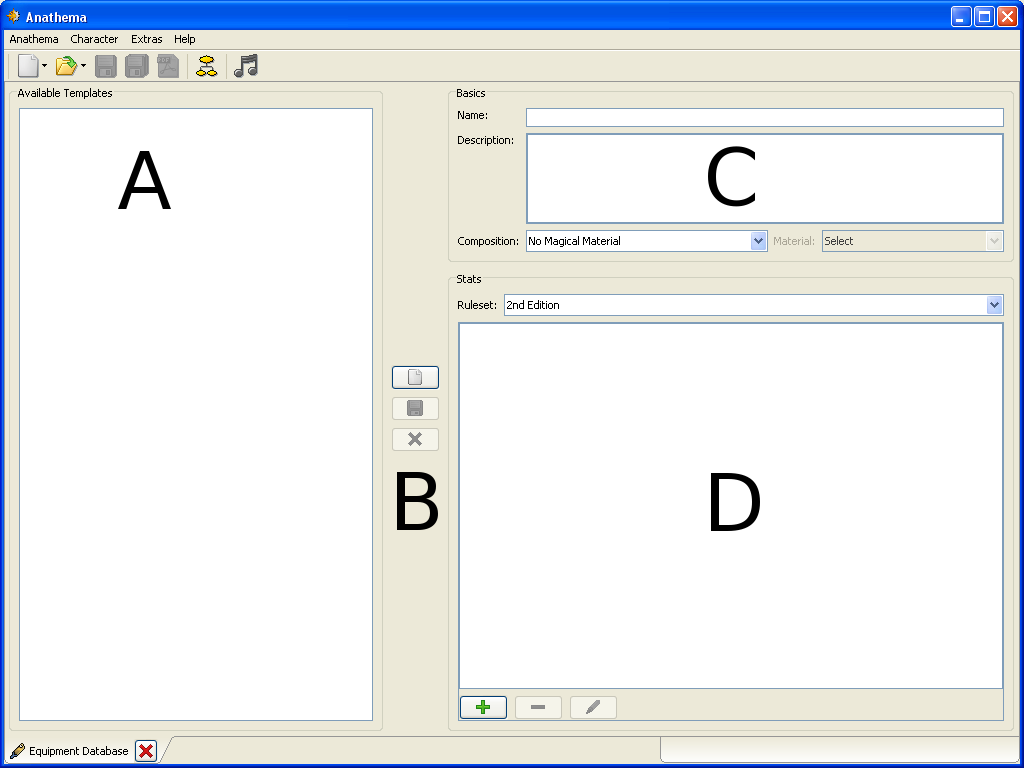
\includegraphics[width=1.00\textwidth]{images/Equipment.png}
	\caption{Equipment Database Screen}
	\label{fig:Equipment}
\end{figure}


The equipment database screen, shown in figure \ref{fig:Equipment}, consists of three parts and a row of buttons. To the left of the panel, there is a vertical list (A), showing all the items in the database. In the center of the screen (B), buttons offer the means for general control - creating, saving and deleting items. The right side is filled with the working area, where items can be edited one at a time.

The working area is composed of two parts, "`Basics"'(C), where the items overall details are handled, and "`Stats"'(D), where you can add statistics to the item. The ruleset selection box functions as both a filter for and a setting, showing only the stats for the ruleset selected and adding newly entered stats to that same ruleset. Do not be alarmed when the data you just entered disappears when you change rules, changing it back will make your hard work reappear.

\section{Basic Items}
To create an item, enter a name, description, and use the composition box to chose if the item is made from one or more magical materials, or not magical.  Artifacts are discussed later, for now lets make a normal item.

Next, chose the ruleset you want to add stats for from the drop down box. Now you are ready to enter the stats of the item.  Using the Template controls at the bottom of the page, press the green + button to open a pop-up window to begin to enter the stats of the item.  Click the icon of the type of item you are making to open the next window so you can enter the numbers.

The next screens will allow you enter the various stats of the item.  You can change the name for the set of statistics, but that is generally only needed if you  will be adding multiple stats. Keep in mind this sub-name will only be displayed if you change it. This comes into play when making complex items, described latter.

Pressing 'Finish' will add the Template to the bottom half of the Database window.
You can then press the Save button in the middle of the window to add the item to the left side panel.  

You can remove existing stats via the '-' icon, and edit them using the pencil button on the right of the row. Thus, you can make changes without starting over.

To enter another new item press the clear button (top middle button that look like a sheet of paper) to clear the right side working area.

You can edit a previous item you have saved by clicking on it on the left side, which will list it on the right side work area were you can add, remove, or edit the templates that compose the item.  Remember to press Save again or your edits will be lost.

\section{Complex Items}
You can create more complex items by creating the base item as normal, then adding additional sets of stats.   

This method allows you to create multi-use items like a Fighting Gauntlet, which can be used to Punch or Clinch by selecting Close Combat but renaming it Punch and enter the stats for Punching.  The add another Close Combat template for clinching, and there you are.

There is no limit to the complexity of items created this way. You should well be able to even create warstriders with various weapons and armour statistics. 

\section{Artifacts}
Once you get beyond making mundane weapons and armor, you enter the complex realm of artifacts. Artifacts differ from mundane items in their material composition, fittingly indicated by the "`composition"' box.

The 3 artifact choices offered are 'Single Material, Fixed', 'Single Material, Variable', and 'Compound'.  

\subsection{Single Material, Variable}
This is the basic option for run-of-the-mill artifacts like those listed in the core book. Choosing it tells the program that this is not a unique item but a class of artifacts. Thus, it will assume that the item receives the defaut boni granted by the magical material, and will automatically add them once the item is equipped.

Going through the steps described previously, you can select the specific items material just before adding it to your character. The program defaults to your characters preferred material.
  
\subsection{Single Material, Fixed}
This option is used to make artifacts that are only available in one Magical Material.
The program assumes that there are special boni involved, and you will need to add the boni (if any) for the magical material when entering the stats for the item. 

Just selecting the Magical Material will not add the appropriate bonus' to the item.

\subsection{Compound}
Compound items are made from more then one Magical Material. Generally, they do neither grant bonus the same way items made from only one material do, nor are they restricted to only one type of exalt.  

Special boni and powers offered by these items will have to be noted in the items description or calculated into their statistics.

\section{Statless Items}
You can make items that are not weapons or armor by just entering the name, description, and selecting the magical material, if any. When you equip a character with these items, they will be printed in the Possessions area on the second page.